\chapter{Uncertainty budget}\label{ch:Uncertainty}
Measuring an hadronic cross section  in LArIAT translates into counting how many hadrons impinged on a slab of argon at a given energy and how many of those hadrons interacted at said energy. So, the key questions here are:
\begin{itemize}
\item[]a) how well do we know the kinetic energy at each point of the tracking? %(Incident Kinetic Energy bins)
\item[]b) how well do we know when the tracking stops? %(Interacting Kinetic Energy bin)
\item[]c) are there any systematic shifts?
\end{itemize}

In order to answer this question, will discuss first a simple scenario  were our beam is 100\% made of pions which arrive as primaries in the TPC (no decay in the beam and no inelastic interaction before the TPC front face). We will then add a layer of complexity by discussing how we handle beamline contamination.

\section{Pure beam of pions}
Assuming a beam of pure pions gets to the TPC, let us explicit some of the variables in the kinetic energy equation \ref{eq:KEj}  to point out the important quantities in the uncertainty budget,

\begin{align}
 E_{j}^{kin} &=  E_{Beam}^{kin}  - E_{loss} - \sum_{i < j} \frac {dE_i}{dx_i}*dx_i\\
                  &=  \sqrt{p^2_{Beam} - m^2_{Beam}} - m_{Beam} - E_{loss} - \sum_{i < j} \frac {dE_i}{dx_i}*dx_i.
\end{align}

\subsection{Uncertainty on $E_{Beam}^{kin}$}
Let us start by discussing the uncertainty on $E_{Beam}^{kin}$. Since we are assuming a beam of pions, the uncertainty on the value of mass of the pion ($m_{Beam}$) as given by the pdg is irrelevant compared to the momentum uncertainties, thus $\delta E_{Beam}^{kin} = \delta p_{Beam}^{kin}$. 
We estimate the momentum uncertainty as follows.

\textcolor{blue}{  
We estimate the uncertainty on a 4-point track. In case of 3-points track, we add an additional 2\% coming from Greg's study. 
Uncertainty on a 4-point track:
\begin{itemize}
\item[-]  Alignment surveys. 1mm misalignment translates to 3\% in overall
\item[-] Doug study dp/p = ~2\% based on field map (docdb 1710)
\item[-] Minerva test beam paper
\end{itemize}
}

\subsection{$E_{loss}$}
We derive an estimate of the energy loss between the beamline momentum measurement and the TPC ($E_{loss}$) from the Monte Carlo using the DDMC pion sample, since this quantity is not  measurable directly on data. We shoot pions from WC4 with the same momentum distribution as in the beamline data and plot the true $E_{loss}$ for that sample. The $E_{loss}$ distribution for the 60A  and 100A pion sample is shown in figure \ref{fig:ELoss60A}, left and right respectively. A clear double peaked structure is visible, which is due to the particles either missing or hitting the HALO paddle: a schematic rendering of this occurrence is  shown in figure \ref{fig:Halo}. The kinematic at WC4 determines the trajectory of a particle and whether or not it will hit the halo paddle. In figure \ref{fig:PxVsXTrue} , we plot the true  $X$ component of the momentum versus the true $X$ position at WC4 for pions missing the halo paddle (left) and for pions hitting the halo paddle (right) for the 60A MC simulation runs -- analogous plots are obtained with the 100A simulation. These distributions can be separated drawing a line in this position-momentum space. 
We use a logistic regression  \cite{agresti2013categorical}  as a classifier to find the best separating line, shown in both plots as the red line. We classify as ``hitting the halo paddle" all pions whose $P_x$ and $X$ are such that $$P_x +0.02* X - 0.4 < 0 $$ and as ``missing the halo  paddle" all pions whose $P_x$ and $X$ are such that $$P_x +0.02*X - 0.4 > 0, $$ where the coefficients of the line are empirically found by the logistic regression estimation. Overall, this simple classifier classifies in the right category (hit or miss) about 86\% of the pion events.
We apply the same classifier on data. We assign  $E_{loss} = 32 \pm 4 $~MeV for events classified as ``hitting the halo paddle"; we assign  $E_{loss} = 24 \pm 3 $~MeV for events classified as ``missing the halo paddle".

%We use the separation of these two distributions to decide what the energy loss for each event on data. 
%Thus,  we assign the value for energy loss is used in the data.


\begin{figure}[hbpt]
\centering
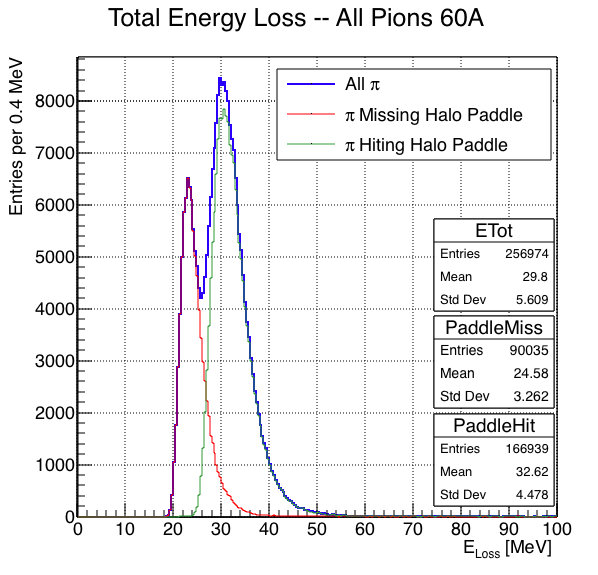
\includegraphics[width=0.45\textwidth]{Chapter-9/Images/E_loss60A.png}
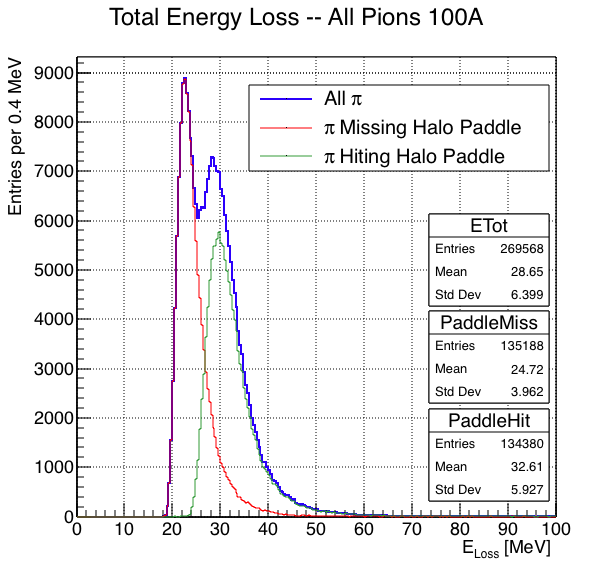
\includegraphics[width=0.45\textwidth]{Chapter-9/Images/E_loss100A.png}
\caption{True energy loss between WC4 and the TPC front face according to the MC simulation of the 60A runs (left) and of the 100A runs (right). The distribution for the whole data sample is shown in blue, the distribution for the pions missing the halo is shown in red, and the distribution for the pions hitting the halo is shown in green.  }
\label{fig:ELoss60A}
\end{figure}

\begin{figure}[hbpt]
\centering
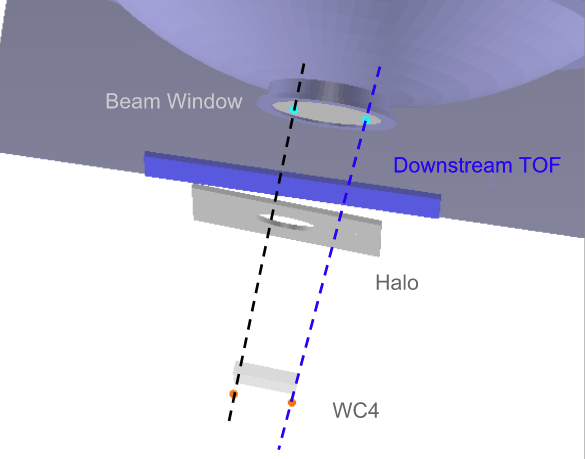
\includegraphics[scale=0.5]{Chapter-9/Images/Halo.png}
\caption{Schematic rendering of the particle path between WC4 and the TPC front face. The paddle with the hollow central circle represents the Halo paddle. We illustrate two possible trajectories: in black, a trajectory that miss the paddle and goes through the hole in the Halo, in blue a trajectory that hits the Halo paddle and goes through the scintillation material.}
\label{fig:Halo}
\end{figure}



\begin{figure}[hbpt]
\centering
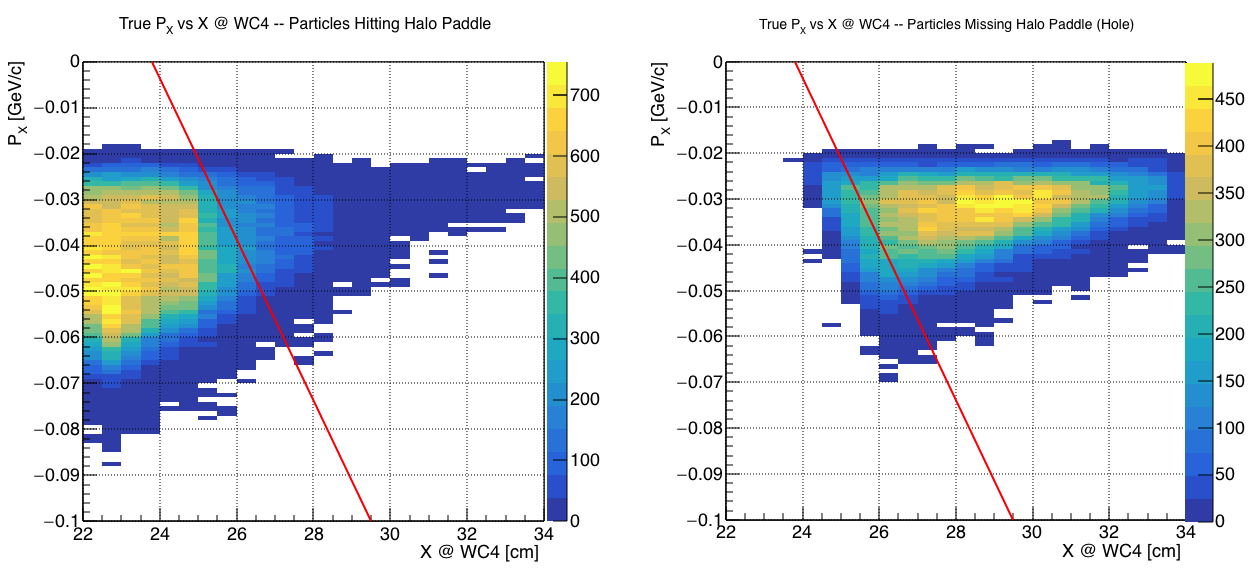
\includegraphics[width=\textwidth]{Chapter-9/Images/PXVsX60A.png}
\caption{Horizontal component of the true momentum vs the horizontal position at WC4 for MC simulated pions of the 60A runs. The plot on the left shows the distribution for pion that miss the halo paddle and the plot on the right shows the distributions for pions that hit the halo. The form of the classifier is overlaid to both plots (red line).}
\label{fig:PxVsXTrue}
\end{figure}





%\textcolor{blue}{ TO DO HERE: make sure we have the geometry right, cause otherwise this correction is meaningless.  With this method, so far we get a mean ~40 MeV, but uncertainty ~7MeV. 
%The trajectory method does not improve uncertainty, why? It's a mystery I don't think we should solve before June :) .
%Back of the envelope material budget calculation:}
%\begin{table}[h!]
%\centering
%\caption{Back of the envelope calculation}
%\label{my-label}
%\begin{tabular}{|l|l|l|l|}
%\hline
%dEdx for MIP, MPV {[}MeV cm$^2$/gr{]} & density {[}g/cm$^3${]} & width {[}cm{]} & E$_{loss}$ {[}MeV{]} \\ \hline
%1.6                                                 & 1.7 (G10)                            & 1.3            & 3.5                   \\
%1.6                                                 & 1.4 (LAr)                            & 1.77           & 4.0                   \\
%1.6                                                 & 7.7 (S.S.)                           & 0.23           & 2.8                   \\
%1.6                                                 & 4.5 (Ti)                             & 0.04           & 0.3                   \\ 
%1.6                                                 & 1.03 (Plastic Sci)                   & 1.1            & 1.8                   \\ \hline
%Total                                               &                                      &                & 12.4                  \\ \hline
%\end{tabular}
%\end{table}



\subsection{Uncertainty on dE/dx and pitch}
We obtain the uncertainty on dE/dx and track pitch by comparing the dE/dx and pitch distributions in data and MC.
\textcolor{blue}{ Currently, MPV MC = 1.70 and MPV DATA = 1.72 MeV/cm (~3\% higher).
TO DO HERE: calculate Argon density from mid-RTD temperature. Compare this  density with MC Argon density. 
Density change  affects dE/dx (in MeV/cm!). Try changing MC density up to ``real one" and see if dEdX agrees between DATA and MC}


\subsection{Uncertainty on track end, aka efficiency correction}
From the MC, we obtain an efficiency correction on the interacting and incident distributions separately. This is done by comparing the MC reconstructed with the true MC deposition on an event by event basis.
This correction is applied bin by bin on the data interacting and incident distributions.
The better our tracking, the smaller this efficiency correction will be. So, step number one is improving the tracking.
\textcolor{blue}{Need to talk to Bruce about this.}
\textcolor{blue}{ I don't understand the angle cut that Dave Schmitz and Jon Paley were so vocal about.}

Now, the key question remains: does the tracking behave in the same way in data and MC? 
We can compare some key plots between reconstructed data and MC which gives us confidence this is true: the track pitch, the tracks straightness and the goodness of fit in data and MC. \textcolor{blue}{ Does such a variable as ``goodness of fit" exists in the tracking? We should ask Bruce.}
